\chapter{Метод моделирования и оптимизации процессов перезагрузки реакторов}

В данной главе будет рассмотрен метод моделирования и оптимизации процессов перезагрузки реактора с использованием методов искусственного интеллекта.
Будут рассмотрены входные и выходные данные для моделирования, а также алгоритмическое исполнение метода.
В конце главы будут представлены преимущества и недостатки данного метода.

\section{Исходные данные для моделирования}

Пусть у нас имеется следующая информация о реакторе и его процессе перезагрузки:
\begin{enumerate}
 \item \textbf{ТА-модель}. 
 ТА-модель представляет собой описание реактора и его процесса ППР в виде автомата или композиции автоматов.
 То есть задано множество состояний реактора, множество операций над реактором, функция перехода, указывающая возможные переходы при из одного конечного состояния в другое при выполнении операции, а также начальное и множество конечных состояний.
 При этом для каждого состояния реактора и каждой операции заданы известные физические характеристики.
 
 \item \textbf{Данные физического моделирования}. 
 Данные физического моделирования представляют собой множество расчетных (или известных) характеристик реактора, соответствующих определенному физическому состоянию реактору.
 Примером таких данных может служить зависимость подкритичности от физической конфигурации активной зоны.
 Данное множество необязательно должно содержать все значения из множества состояния реактора.
 При этом могут использоваться данные прошлых кампаний.
 Также для этого каждого значения множества должна быть указана допустимость таких расчетных характеристик.
 
 \item \textbf{Функция оптимизации}.
 Функция оптимизации --- весовая функция для характеристик операций, проводимых над реактором.
 Она требуется для изменения значимости различных факторов при проведении оптимизации.
 Поиск оптимального порядка будет производится по минимальным значениям данной функции. 
\end{enumerate}

Обработав исходные данные, метод должен представить на выходе оптимальный с точки зрения функции оптимизации порядок проведения перезагрузки реактора. 
При этом искомый порядок не должен содержать физически недопустимых состояний (см. рис.~\ref{pic:method-blackbox}).


\begin{figure}[ht]
\center{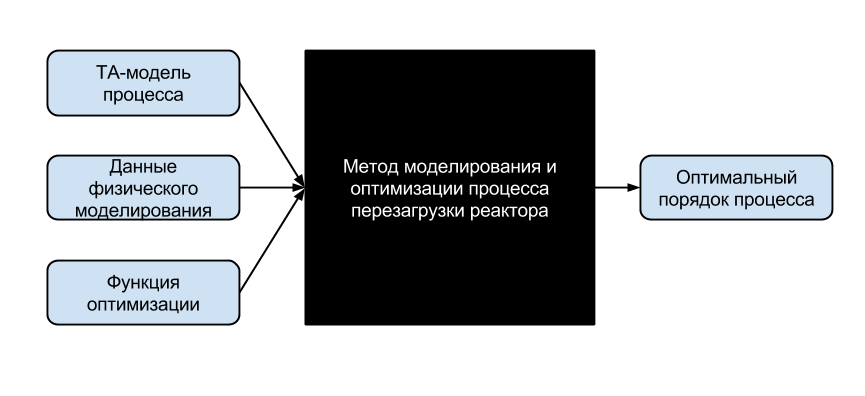
\includegraphics[width=\linewidth]{method-blackbox}}
\caption{Входные и выходные данные метода моделирования и оптимизации}
\label{pic:method-blackbox}
\end{figure}

\section{Описание метода моделирования и оптимизации}

Рассмотрим работу метода моделирования и оптимизации перегрузки реактора (см. рис.~\ref{pic:method-whitebox}).

\begin{enumerate}
 \item Искусственная нейронная сеть обучается на данных физического моделирования.
 После успешного обучения нейронная сеть становится способна аппроксимировать расчетные характеристики реактора на основе физического состояния реактора, а также выносить решение о допустимости состояния.
 
 \item Множество состояний ТА-модели реактора поэлементно подается в качестве входного вектора искусственной нейронной сети.
 ИНС делит множество на допустимые и недопустимые состояния.
 Допустимые состояния становятся узлами графа, а недопустимые --- отбрасываются.
 
 \item Между узлами графа проводятся направленные ребра на основе множества операции и функции перехода.
 Таким образом после завершения операции имеется граф переходов между допустимыми состояниями.
 
 \item В полученном графе запускается алгоритм поиска А*.
 Алгоритм производит поиск кратчайшего пути между начальным состоянием и каждым состоянием из множества конечных.
 При этом в качестве эвристической функции используется функция оптимизации.
 
 \item По завершению работы алгоритма поиска имеется множество путей, ведущих кратчайшим путем к каждому из конечных состояний.
 Путь с минимальным значением функции оптимизации является искомым.
 
\end{enumerate}

\begin{figure}[ht]
\center{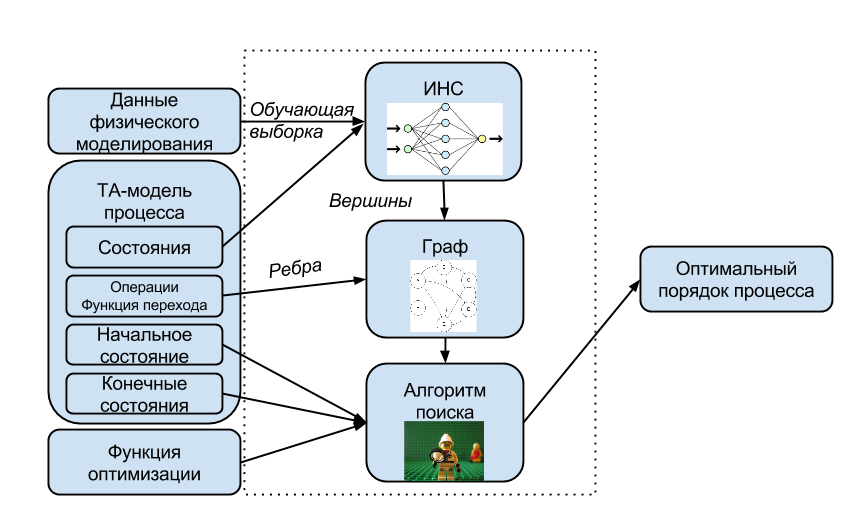
\includegraphics[width=\linewidth]{method-whitebox}}
\caption{Метод моделирования и оптимизации}
\label{pic:method-whitebox}
\end{figure}

Полученные в результате работы метода порядок перезагрузки необходимо проверить сертифицированными средствами физического моделирования реактора.


\section{Преимущества и недостатки метода}

К преимуществам данного метода относятся:
\begin{itemize}
 \item [-] \textbf{Универсальность}.
 Данный метод не ограничивается одним типом реакторов.
 При наличии исходных данных метод можно применить к любому типу реактора.
 В перспективе метод можно будет применить к любым системам, описываемым формализмом ТА-моделей
 
 \item [-] \textbf{Гибкость}. 
 Задаваемая функция оптимизации позволяет оптимизировать одну и ту же ТА-модель по различным параметрам.
 Для этого не требуется изменение метода и/или модели.
 
 \item [-] \textbf{Высокая скорость работы}.
 За счет применения информированного алгоритма поиска и искусственных нейронных сетей для аппроксимации физических характеристик метод имеет приемлемую вычислительную сложность.
\end{itemize}

К недостаткам данного метода относятся:
\begin{itemize}
 \item [-] \textbf{Сложность описания ТА-модели}.
 Для построения ТА-модели реактора в нужной детализации требуется достаточно много усилий.
 Это увеличивает вероятность ошибок в задании модели реактора, а, следовательно, в расчетах.
 
 \item [-] \textbf{Возможность ошибки аппроксимации в ИНС}.
 ИНС может иметь ошибки аппроксимации, связанные с переобучением или отсутствием информации об особенностях  данной области аппроксимации.
\end{itemize}

